\begin{frame}
\centering
\textcolor{red}{\textit{\textbf{Temporal semantic} OS system based on heat maps}}
\end{frame}
%========================================== ############# ======================================================
%========================================== ############# ======================================================
%========================================== ############# ======================================================
\begin{frame}{Introduction}
	\begin{columns}[T]
	\column{.55\textwidth}
		\begin{itemize}[<+->]
			\item \textbf{Service robots} and their use in indoor environments
			\item Number of older people living at home is increasing
			\item The \textbf{OS task} for young and old people
			\item \textbf{Brute-force OS} strategy \textbf{is not practical} 
			\item \textbf{Visual sensors} embedded in robots
			\item The \textbf{advantages} of visual sensors for the \textbf{OS problem}
		\end{itemize}
	\column{.45\textwidth}
		\centering
		\begin{figure}
			\includegraphics[width=.9\linewidth]{figs/care_o_bot.png}
			\caption{\tiny Evolution of the Care-O-bot.\footnotemark[15]}			 		 
		\end{figure}			
	\end{columns}
	\footnotetext[15]{\tiny Figure extracted from \url{care-o-bot.de/en/care-o-bot-3/history.html}.}			
\end{frame}
%========================================== ############# ======================================================
%========================================== ############# ======================================================
%========================================== ############# ======================================================
\begin{frame}{Humans-object interaction}
	\begin{itemize}[<+->]
		\item \textbf{Humans activities} have an influence in the \textbf{objects' placement}
		\item Most of the \textbf{robotic approaches ignores semi-dynamic or dynamic objects}
		\item \textbf{Understanding} how the \textbf{objects are moved} throughout a period of time \textbf{may help in the OS problem}
		\item \textbf{Realistic} (the environment changes) and \textbf{customized} (adapts to the local habits and routines) \textbf{OS system}
	\end{itemize}
\end{frame}
%========================================== ############# ======================================================
%========================================== ############# ======================================================
%========================================== ############# ======================================================
\begin{frame}{Proposal and contributions}
	\begin{columns}[T]
	\column{.5\textwidth}
		\begin{itemize}[<+->]
			\item \textbf{Semantic temporal OS system} for indoor environment
			\item Self-contained OS system
			\item Advantages of \textbf{semantic information} from \textbf{dynamic environments}
			\item Searches based on the \textbf{request hour}
		\end{itemize}
	\column{.5\textwidth}
		\centering
		\begin{figure}
			\includegraphics[width=.8\linewidth]{figs/general_idea_300dpi.png}
			\caption{\tiny General idea of our OS system.}
		\end{figure}			
	\end{columns}	
\end{frame}
%========================================== ############# ======================================================
%========================================== ############# ======================================================
%========================================== ############# ======================================================
\begin{frame}{System overview}
	\begin{columns}[T]
	\column{.3\textwidth}
		\begin{itemize}
			\item Two modes OS system:
			\begin{itemize}
				\item \textbf{Recording} mode
			\end{itemize}
		\end{itemize}
	\column{.7\textwidth}
		\centering
		\begin{figure}
			\includegraphics[width=.8\linewidth]{figs/system_overview_shade.png}
			\caption{\tiny Flow chart of our Semantic, Temporal OS system.}
		\end{figure}			
	\end{columns}	
\end{frame}
%========================================== ############# ======================================================
%========================================== ############# ======================================================
%========================================== ############# ======================================================
\begin{frame}[noframenumbering]{System overview}
	\begin{columns}[T]
	\column{.3\textwidth}
		\begin{itemize}
			\item Two modes OS system:
			\begin{itemize}
				\item \textbf{Recording} mode
				\item \textbf{Requesting} mode
			\end{itemize}
		\end{itemize}
	\column{.7\textwidth}
		\centering
		\begin{figure}
			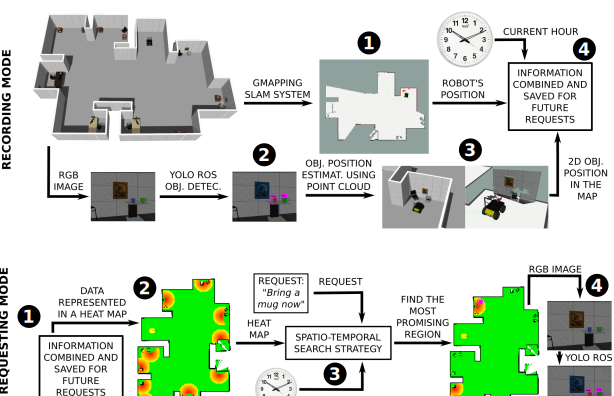
\includegraphics[width=.8\linewidth]{figs/system_overview.png}
			\caption{\tiny Flow chart of our Semantic, Temporal OS system.}
		\end{figure}			
	\end{columns}	
\end{frame}
%========================================== ############# ======================================================
%========================================== ############# ======================================================
%========================================== ############# ======================================================
\begin{frame}{The OS system}
	\begin{columns}[T]
	\column{.38\textwidth}
	\begin{itemize}
		\item \textbf{Heat map}
		\begin{itemize}
			\item Based on the 2D grid map
			\item Circular kernel
		\end{itemize}
	\end{itemize}
	\column{.65\textwidth}
		\centering
		\begin{figure}
			\includegraphics[width=.8\linewidth]{figs/environment_2Dgrid_heatmap_kernel.png}
			\caption{\tiny Simulated world, its 2D grid map, and the heat map computed by our OS system.}
		\end{figure}			
	\end{columns}	
\end{frame}
%========================================== ############# ======================================================
%========================================== ############# ======================================================
%========================================== ############# ======================================================
\begin{frame}[noframenumbering]{The OS system}
	\begin{columns}[T]
	\column{.4\textwidth}
		\begin{itemize}
			\item \textbf{Heat map}
			\begin{itemize}
				\item Based on the 2D grid map
				\item Circular kernel
			\end{itemize}			
			\item Kernel \textbf{angle reduction}
		\end{itemize}
	\column{.32\textwidth}
		\centering
		\begin{figure}
			\begin{subfigure}{.8\columnwidth}
				\centering
				\includegraphics[width=1\linewidth]{figs/bad_robot_placement_1.png}
%				\caption{\tiny backgrounds​.}
			\end{subfigure}
			\begin{subfigure}{.8\columnwidth}			
				\centering			
				\includegraphics[width=1\linewidth]{figs/bad_robot_placement_2.png}			
%				\caption{\tiny backgrounds​.}				
			\end{subfigure}
			\caption{\tiny Bad robot placement.}			
		\end{figure}		
	\column{.32\textwidth}
		\centering
		\begin{figure}
			\begin{subfigure}{.8\columnwidth}
				\includegraphics[width=1.05\linewidth]{figs/good_robot_placement_1.png}
%				\caption{\tiny Signs on primary routes, green backgrounds​.}
			\end{subfigure}
			\begin{subfigure}{.8\columnwidth}		
				\centering						
				\includegraphics[width=1.05\linewidth]{figs/good_robot_placement_2.png}			
%				\caption{\tiny backgrounds​.}								
			\end{subfigure}
				\caption{\tiny Good robot placement.}											
		\end{figure}				
	\end{columns}	
\end{frame}
%========================================== ############# ======================================================
%========================================== ############# ======================================================
%========================================== ############# ======================================================
\begin{frame}[noframenumbering]{The OS system}
	\begin{columns}[T]
	\column{.4\textwidth}
	\begin{itemize}
			\item \textbf{Heat map}
			\begin{itemize}
				\item Based on the 2D grid map
				\item Circular kernel
			\end{itemize}			
			\item Kernel \textbf{angle reduction}
		\item \textbf{Inverted kernel}
	\end{itemize}
	\column{.6\textwidth}
		\centering
		\begin{figure}
			\begin{subfigure}{.48\columnwidth}
				\centering
				\includegraphics[width=1\linewidth]{figs/normal_kernel_complete_reduced.png}
				\caption{\tiny Heat map with the normal kernel.}
			\end{subfigure}
			\begin{subfigure}{.48\columnwidth}		
				\centering			
				\includegraphics[width=1\linewidth]{figs/inversed_kernel_complete_reduced.png}			
				\caption{\tiny Heat map with the inverted kernel.}				
			\end{subfigure}
			\caption{\tiny Illustration of the different kernels and the Heat map.}
		\end{figure}		
	\end{columns}	
\end{frame}
%========================================== ############# ======================================================
%========================================== ############# ======================================================
%========================================== ############# ======================================================
\begin{frame}{The OS system}
	\begin{columns}[T]
	\column{.3\textwidth}
	\begin{itemize}
		\item Goal computation
		\begin{itemize}
			\item \textbf{Warmest area}
		\end{itemize}
	\end{itemize}
	\column{.7\textwidth}
		\centering
		\begin{figure}
			\centering
			\includegraphics[width=.65\linewidth]{figs/inversed_kernel_complete_reduced.png}
			\caption{\tiny Inverted and reduced kernel for goal computation.}
		\end{figure}			
	\end{columns}	
\end{frame}
%========================================== ############# ======================================================
%========================================== ############# ======================================================
%========================================== ############# ======================================================
\begin{frame}{Experiments and results}
	\begin{columns}[T]
	\column{.4\textwidth}
		\centering	
		\begin{itemize}
			\item HH106 dataset\footnotemark[16]
		\end{itemize}
	\column{.6\textwidth}
		\centering
		\begin{figure}
%			\begin{subfigure}{.8\columnwidth}
				\includegraphics[width=.6\linewidth]{figs/hh106sensor_map.png}
				\caption{\tiny The floorplan of the single-resident apartment from the HH106 dataset.}
		\end{figure}		
	\end{columns}	
		\footnotetext[16]{\tiny Dataset available at \url{http://casas.wsu.edu/datasets/}.}
\end{frame}
%========================================== ############# ======================================================
%========================================== ############# ======================================================
%========================================== ############# ======================================================
\begin{frame}[noframenumbering]{Experiments and results}
	\begin{columns}[T]
	\column{.4\textwidth}
		\begin{itemize}
			\item HH106 dataset\footnotemark[16]	
			\item Simulation setup and maps
		\end{itemize}
	\column{.6\textwidth}
		\centering
		\begin{figure}
%			\begin{subfigure}{.8\columnwidth}
				\includegraphics[width=.45\linewidth]{figs/simulated_environment.png}
				\includegraphics[width=.25\linewidth]{figs/husky_robot.png}
				\caption{\tiny Environment and robot used in simulation.}
		\end{figure}		
	\end{columns}					
		\footnotetext[16]{\tiny Dataset available at \url{http://casas.wsu.edu/datasets/}.}	
\end{frame}
%========================================== ############# ======================================================
%========================================== ############# ======================================================
%========================================== ############# ======================================================
\begin{frame}[noframenumbering]{Experiments and results}
	\begin{columns}[T]
	\column{.4\textwidth}
		\begin{itemize}
			\item HH106 dataset\footnotemark[16]		
			\item Simulation setup and maps
			\item Two other OS systems:
			\begin{itemize}
				\item Brute Force
				\item Last Seen 
			\end{itemize}
		\end{itemize}
	\column{.6\textwidth}
		\centering
		\begin{figure}
%			\begin{subfigure}{.8\columnwidth}
				\includegraphics[width=.6\linewidth]{figs/brute_force_route2.png}
				\caption{\tiny The robot’s route for the Brute Force OS approach.}
		\end{figure}		
	\end{columns}		
		\footnotetext[16]{\tiny Dataset available at \url{http://casas.wsu.edu/datasets/}.}			
\end{frame}
%========================================== ############# ======================================================
%========================================== ############# ======================================================
%========================================== ############# ======================================================
\begin{frame}[noframenumbering]{Experiments and results}
	\begin{columns}[T]
	\column{.4\textwidth}
		\begin{itemize}
			\item HH106 dataset\footnotemark[16]		
			\item Simulation setup and maps
			\item Two other OS systems:
			\begin{itemize}
				\item Brute Force
				\item Last Seen 
			\end{itemize}
			\item The \textbf{shorter} the \textbf{traveled distance}, the \textbf{better}
		\end{itemize}
	\column{.6\textwidth}
		\centering
		\begin{figure}
%			\begin{subfigure}{.8\columnwidth}
				\includegraphics[width=.6\linewidth]{figs/brute_force_route2.png}
				\caption{\tiny The robot’s route for the Brute Force OS approach.}				
		\end{figure}		
	\end{columns}		
		\footnotetext[16]{\tiny Dataset available at \url{http://casas.wsu.edu/datasets/}.}			
\end{frame}
%========================================== ############# ======================================================
%========================================== ############# ======================================================
%========================================== ############# ======================================================
\begin{frame}{Experiments and results}
	\begin{columns}[T]
	\column{.4\textwidth}
		\begin{itemize}
			\item The HH106 dataset:
			\begin{itemize}
				\item \textbf{Long-term dataset} (60 days)
				\item \textbf{Motion sensors} provide the \textbf{human location} at different hours of the day
				\item The\textbf{ person mimics an object} that is moved many times every day
				\item \textbf{59 days} of data for the \textbf{Recording mode}
			\end{itemize}			 			 
		\end{itemize}
	\column{.6\textwidth}
	\vspace{-.7cm}
\begin{table}
\tiny
\centering
%\caption[The 59 days data from HH106 used by our OS system.]{The 59 days data from HH106 used by our OS system.}
\begin{tabular}{c|cccccccc}\hline %
\multirow{2}{*}{\textbf{\begin{tabular}[c]{@{}c@{}}Daily \\ Hours\end{tabular}}} & \multicolumn{8}{c}{\textbf{Locations}} \\
                                      & \textbf{W.A.} & \textbf{Liv.R.}    & \textbf{Kit.}    & \textbf{BedR.}    & \textbf{Chair}    & \textbf{Din.R.}    & \textbf{BathR.} & \textbf{O.D.}  \\ \hline
00 & 0 & 2 & 1 & 21 & 0 & 1 & 3 & 2 \\\hline
01 & 2 & 1 & 3 & 20 & 0 & 1 & 1 & 2 \\\hline
02 & 3 & 5 & 1 & 29 & 0 & 0 & 0 & 0 \\\hline
03 & 1 & 4 & 3 & 24 & 0 & 0 & 0 & 2 \\\hline
04 & 3 & 0 & 1 & 28 & 0 & 2 & 0 & 1 \\\hline
05 & 0 & 1 & 2 & 35 & 0 & 1 & 0 & 1 \\\hline
06 & 1 & 3 & 3 & 31 & 0 & 1 & 4 & 10 \\\hline
07 & 1 & 4 & 4 & 10 & 0 & 6 & 5 & 7 \\\hline
08 & 3 & 2 & 4 & 4 & 1 & 14 & 8 & 5 \\\hline
09 & 6 & 2 & 1 & 1 & 0 & 15 & 3 & 12 \\\hline
10 & 3 & 1 & 1 & 3 & 0 & 3 & 11 & 19 \\\hline
11 & 6 & 3 & 7 & 2 & 0 & 3 & 5 & 13 \\\hline
12 & 7 & 3 & 2 & 1 & 1 & 14 & 4 & 12 \\\hline
13 & 5 & 8 & 3 & 0 & 5 & 4 & 6 & 13 \\\hline
14 & 4 & 5 & 1 & 0 & 2 & 5 & 4 & 16 \\\hline
15 & 9 & 4 & 5 & 0 & 0 & 4 & 2 & 17 \\\hline
16 & 16 & 5 & 4 & 1 & 2 & 6 & 2 & 7 \\\hline
17 & 16 & 2 & 4 & 2 & 0 & 9 & 1 & 7 \\\hline
18 & 21 & 4 & 3 & 1 & 0 & 3 & 2 & 13 \\\hline
19 & 14 & 5 & 2 & 1 & 0 & 4 & 2 & 11 \\\hline
20 & 13 & 8 & 2 & 0 & 0 & 6 & 7 & 2 \\\hline
21 & 14 & 3 & 0 & 8 & 0 & 13 & 8 & 1 \\\hline
22 & 1 & 3 & 2 & 37 & 0 & 1 & 6 & 0 \\\hline
23 & 1 & 2 & 0 & 34 & 1 & 1 & 1 & 0 \\\hline
\textbf{Total} & 150 & 80 & 59 & 293 & 12 & 117 & 85 & 173
\end{tabular}
%\label{tab:all_days_hh106}
\end{table}	
	\end{columns}
\end{frame}
%========================================== ############# ======================================================
%========================================== ############# ======================================================
%========================================== ############# ======================================================
\begin{frame}{Experiments and results}
	\begin{columns}[T]
	\column{.4\textwidth}
		\begin{itemize}
			\item The HH106 dataset
			\begin{itemize}
				\item The \textbf{60th day} as the \textbf{ground-truth}
			\end{itemize}			 
		\end{itemize}
	\column{.6\textwidth}
	\vspace{-.5cm}
	\hspace{2cm}
\begin{table}
\tiny
\centering
%\caption[The data from the last day of HH106 used to test our OS system.]{The data from the last day of HH106 used to test our OS system.}
\begin{tabular}{c|cccccccc}\hline
\multirow{2}{*}{\textbf{\begin{tabular}[c]{@{}c@{}}Daily \\ Hours\end{tabular}}}  & \multicolumn{8}{c}{\textbf{Locations}}\\
      & \textbf{W.A.} & \textbf{Liv.R.}    & \textbf{Kit.}    & \textbf{BedR.}    & \textbf{Chair}    & \textbf{Din.R.}    & \textbf{BathR.} & \textbf{O.D.}  \\\cline{1-9}
%00 & 0 & 0 & 0 & 0 & 0 & 0 & 0 & 0
%\\\midrule
01 & 0 & 0 & 0 & 1 & 0 & 0 & 0 & 0 \\\hline
02 & 0 & 0 & 0 & 1 & 0 & 0 & 0 & 0 \\\hline
%03 & 0 & 0 & 0 & 0 & 0 & 0 & 0 & 0
%\\\midrule
04 & 0 & 0 & 0 & 1 & 0 & 0 & 0 & 0 \\\hline
05 & 0 & 0 & 0 & 1 & 0 & 0 & 0 & 0 \\\hline
06 & 0 & 0 & 0 & 0 & 0 & 0 & 0 & 1 \\\hline
%07 & 0 & 0 & 0 & 0 & 0 & 0 & 0 & 0
%\\\midrule
08 & 0 & 0 & 1 & 0 & 0 & 0 & 0 & 0 \\\hline
09 & 0 & 0 & 0 & 0 & 0 & 1 & 0 & 0 \\\hline
10 & 0 & 0 & 0 & 0 & 0 & 0 & 0 & 1 \\\hline
11 & 0 & 0 & 0 & 0 & 0 & 0 & 1 & 0 \\\hline
12 & 1 & 0 & 0 & 0 & 0 & 0 & 0 & 0 \\\hline
13 & 0 & 0 & 0 & 0 & 0 & 0 & 0 & 1 \\\hline
14 & 0 & 1 & 0 & 0 & 0 & 0 & 0 & 0 \\\hline
15 & 1 & 0 & 0 & 0 & 0 & 0 & 0 & 0 \\\hline
16 & 0 & 0 & 0 & 0 & 0 & 0 & 0 & 1 \\\hline
%17 & 0 & 0 & 1 & 0 & 0 & 0 & 0 & 0
%\\\midrule
18 & 1 & 0 & 0 & 0 & 0 & 0 & 0 & 0 \\\hline
19 & 1 & 0 & 0 & 0 & 0 & 0 & 0 & 0 \\\hline
20 & 0 & 0 & 0 & 0 & 0 & 0 & 0 & 1 \\\hline
21 & 0 & 0 & 0 & 1 & 0 & 0 & 0 & 0 \\\hline
22 & 0 & 0 & 0 & 1 & 0 & 0 & 0 & 0 \\\hline
23 & 0 & 0 & 0 & 1 & 0 & 0 & 0 & 0 \\\hline
\textbf{Total} & 4 & 1 & 1 & 7 & 0 & 1 & 1 & 5
\end{tabular}
\label{tab:first_day_hh106}
\end{table}	
	\end{columns}
\end{frame}
%========================================== ############# ======================================================
%========================================== ############# ======================================================
%========================================== ############# ======================================================
\begin{frame}{Experiments and results}
	\begin{columns}[T]
	\column{.4\textwidth}
		\begin{itemize}
			\item The HH106 dataset
			\begin{itemize}
				\item \textbf{Estimations} based on the \textbf{59 days}
				\item Requests for five different hours
			\end{itemize}
		\end{itemize}
	\column{.65\textwidth}
	\vspace{-.5cm}
\begin{table}
\tiny
\centering
%\caption[The human's presence estimation from our OS system.]{The human's presence estimation from our OS system.}
\begin{tabular}{c|cccccccc}\hline
\textbf{Req.}  & \multicolumn{8}{c}{\textbf{Locations}}\\
\textbf{Hours}  & \textbf{W.A.} & \textbf{Liv.R.}    & \textbf{Kit.}    & \textbf{BedR.}    & \textbf{Chair}    & \textbf{Din.R.}    & \textbf{BathR.} & \textbf{O.D.}  \\\cline{1-9}
01 & 59.92 & 35.42 & 24.92 & \textbf{219.66} & 2.0 & 43.5 & 34.92 & 51.25 \\\hline
10 & 67.42 & 38.58 & 33.83 & 106.08 & 7.83 & 69.58 & 48.33 & \textbf{115.00} \\\hline
16 & 106.41 & 46.58 & 32.5 & 76.25 & 8.83 & 68.92 & 46.66 & \textbf{109.66} \\\hline
18 & \textbf{108.41} & 46.08 & 29.66 & 101.25 & 7.16 & 61.75 & 42.66 & 93.50 \\\hline
22 & 82.58 & 41.42 & 25.16 & \textbf{186.92} & 4.16 & 47.41 & 36.66 & 58.00 \\\hline
\end{tabular}
%\label{tab:all_days_hh106_estimations}
\end{table}
	\end{columns}
\end{frame}
%========================================== ############# ======================================================
%========================================== ############# ======================================================
%========================================== ############# ======================================================
\begin{frame}{Experiments and results}
	\begin{columns}[T]
		\column{.3\textwidth}
		\begin{itemize}
			\item Patterns:
			\begin{itemize}
				\item Static
				\item Static-Inv
				\item Mobile
				\item Mobile-Inv			
				\item Shift
			\end{itemize}
		\end{itemize}
		\column{.6\textwidth}
		\begin{table}
		\tiny
		\centering
%		\caption[Mug's position recorded in five setups by the recording mode of our proposal.]{Mug's position recorded in five setups by the recording mode of our proposal.}
		\begin{tabular}{c|cccccccccc}\hline
		\multirow{3}{*}{Pattern}                                         & \multicolumn{10}{c}{Recording hours}\\
		                                         & \multicolumn{5}{c}{Morning} & \multicolumn{5}{c}{Evening}\\
		  & 3 & 5 & 7 & 9 & 11~ & ~15 & 17 & 19 & 21 & 23  \\\hline
		\textit{Static} & A & A & A & A & A~ & ~H & H & H & H & H
		\\\hline
		\textit{Static-Inv} & H & H & H & H & H~ & ~A & A & A & A & A
		\\\hline
		\textit{Mobile} & A & H & A & H & A~ & ~H & A & H & A & H
		\\\hline
		\textit{Mobile-Inv} & H & A & H & A & H~ & ~A & H & A & H & A
		\\\hline
		\textit{Shift} & H & H & H & H & A~ & ~A & A & A & A & H
		%\\\midrule
		%6 & H & H & H & H & A~ & ~A & A & A & A & H
		\\\hline
		\end{tabular}
%		\label{tab:objects_presence_setups}
		\end{table}		
%		\column{.4\textwidth}	
\\
		\begin{columns}
		\column{.6\textwidth}
\begin{table}[!h]
\tiny
\centering
%\caption[Ground-truth of the mug's position for every setup according to the requesting hours.]{Ground-truth of the mug's position for every setup according to the requesting hours.}
\begin{tabular}{c|cc}\hline
\multirow{2}{*}{Pattern}                                           & \multicolumn{2}{c}{Requesting hours}\\
     & ~~~12           & 00  \\\hline
\textit{Static} & ~~~A & H
\\\hline
\textit{Static-Inv} & ~~~H & A
\\\hline
\textit{Mobile} & ~~~A & H
\\\hline
\textit{Mobile-Inv} & ~~~H & A
\\\hline
\textit{Shift} & ~~~A & H
\\\hline
\end{tabular}
\label{tab:ground_truth_mugs}
\end{table}		
		\column{.4\textwidth}
		\begin{figure}
%			\begin{subfigure}{.8\columnwidth}
				\includegraphics[width=.85\linewidth]{figs/brute_force_route2.png}
		\end{figure}			
		\end{columns}				
	\end{columns}
\end{frame}
%========================================== ############# ======================================================
%========================================== ############# ======================================================
%========================================== ############# ======================================================
\begin{frame}[noframenumbering]{Experiments and results}
	\begin{columns}[T]
		\column{.3\textwidth}
		\begin{itemize}
			\item Results for each pattern:
			\begin{itemize}
				\item Static
				\item Static-Inv
				\item Mobile
				\item Mobile-Inv					
			\end{itemize}
		\end{itemize}
		\column{.85\textwidth}
%			\centering
			\begin{figure}
				\vspace{-.5cm}			
				\begin{subfigure}{.4\columnwidth}
					\includegraphics[width=.9\linewidth]{figs/static_setup.png}
					\caption{\tiny Static pattern.}
				\end{subfigure}
				\begin{subfigure}{.4\columnwidth}					
					\includegraphics[width=.9\linewidth]{figs/static_inv_setup.png}					
					\caption{\tiny Static-Inv pattern.}
				\end{subfigure}\\
				\begin{subfigure}{.4\columnwidth}
					\includegraphics[width=.9\linewidth]{figs/mobile_setup.png}
					\caption{\tiny Mobile pattern.}
				\end{subfigure}
				\begin{subfigure}{.4\columnwidth}					
					\includegraphics[width=.9\linewidth]{figs/mobile_inv_setup.png}					
					\caption{\tiny Mobile-Inv pattern.}
				\end{subfigure}				
					\caption{\tiny Results for the first four patterns.}
			\end{figure}					
	\end{columns}				
\end{frame}
%========================================== ############# ======================================================
%========================================== ############# ======================================================
%========================================== ############# ======================================================
%\begin{frame}[noframenumbering]{Experiments and results}
%	\begin{columns}[T]
%		\column{.3\textwidth}
%		\begin{itemize}
%			\item Results for each map:
%			\begin{itemize}
%%				\item Static
%%				\item Static-Inv
%				\item Mobile
%				\item Mobile-Inv			
%			\end{itemize}
%		\end{itemize}
%		\column{.7\textwidth}
%			\centering
%			\begin{figure}
%	%			\begin{subfigure}{.8\columnwidth}
%					\includegraphics[width=.5\linewidth]{figs/mobile_setup.png}~
%					\includegraphics[width=.5\linewidth]{figs/mobile_inv_setup.png}	
%			\end{figure}		
%	\end{columns}				
%\end{frame}
%========================================== ############# ======================================================
%========================================== ############# ======================================================
%========================================== ############# ======================================================
\begin{frame}[noframenumbering]{Experiments and results}
	\begin{columns}[T]
		\column{.3\textwidth}
		\begin{itemize}
			\item Results for each map:
			\begin{itemize}
%				\item Static
%				\item Static-Inv
%				\item Mobile
%				\item Mobile-Inv			
				\item Shift
				\item All combined			
			\end{itemize}
		\end{itemize}
		\column{.85\textwidth}
%			\centering
			\begin{figure}
				\vspace{-.5cm}			
				\hspace{-.5cm}							
				\begin{subfigure}{.4\columnwidth}
					\centering				
					\includegraphics[width=.9\linewidth]{figs/shift_setup.png}
					\caption{\tiny Shift pattern.}
				\end{subfigure}
				\begin{subfigure}{.4\columnwidth}					
					\centering				
					\includegraphics[width=.9\linewidth]{figs/all_combined_setup.png}					
					\caption{\tiny All patterns combined.}
				\end{subfigure}\\
				\begin{subfigure}{.4\columnwidth}
					\centering				
					\includegraphics[width=.4\linewidth]{figs/BF_roomH2.png}
					\caption{\tiny Brute Force search.}
				\end{subfigure}
%				\begin{subfigure}{.4\columnwidth}	
%					\centering									
%					\includegraphics[width=.4\linewidth]{figs/OUR_roomA_roomH2.png}					
%					\caption{\tiny Our OS system.}
%				\end{subfigure}				
					\caption{\tiny Results for the two other patterns.}
			\end{figure}	

%		
%		\column{.7\textwidth}
%			\centering
%			\begin{figure}
%	%			\begin{subfigure}{.8\columnwidth}
%					\includegraphics[width=.5\linewidth]{figs/.png}
%			\end{figure}		
	\end{columns}				
\end{frame}
%========================================== ############# ======================================================
%========================================== ############# ======================================================
%========================================== ############# ======================================================
%\begin{frame}[noframenumbering]{Experiments and results}
%	\begin{columns}[T]
%		\column{.3\textwidth}
%		\begin{itemize}
%			\item Results for each map:
%			\begin{itemize}
%%				\item Static
%%				\item Static-Inv
%%				\item Mobile
%%				\item Mobile-Inv			
%%				\item Shift
%				\item Mobile-Inv modified
%			\end{itemize}
%		\end{itemize}
%		
%	\column{.3\textwidth}
%		\centering
%		\begin{figure}
%%			\begin{subfigure}{.8\columnwidth}
%				\includegraphics[width=.8\linewidth]{figs/mobile_inv_modified_setup.png}
%		\end{figure}						
%	\column{.3\textwidth}
%		\centering	
%		\begin{figure}			
%%				\caption{\tiny Signs on primary routes, green backgrounds​.}
%%			\end{subfigure}
%%			\begin{subfigure}{.8\columnwidth}		
%				\includegraphics[width=.7\linewidth]{figs/OUR_roomA_roomH2.png}			
%%			\end{subfigure}
%		\end{figure}				
%		
%%		\column{.7\textwidth}
%%			\centering
%%			\begin{figure}
%%	%			\begin{subfigure}{.8\columnwidth}
%%					\includegraphics[width=.35\linewidth]{figs/.png}
%%			\end{figure}		
%	\end{columns}				
%\end{frame}
%========================================== ############# ======================================================
%========================================== ############# ======================================================
%========================================== ############# ======================================================
\begin{frame}[noframenumbering]{Experiments and results}
	\begin{columns}[T]
		\column{.3\textwidth}
		\begin{itemize}
			\item Results for each map:
			\begin{itemize}
				\item Modified Mobile-Inv pattern
			\end{itemize}
		\end{itemize}
		\column{.7\textwidth}
			\begin{figure}
				\vspace{-.5cm}			
				\hspace{-.5cm}							
				\begin{subfigure}{.4\columnwidth}
					\centering				
					\includegraphics[width=.88\linewidth]{figs/mobile_inv_modified_setup.png}
					\caption{\tiny Modified Mobile-Inv pattern.}
				\end{subfigure}
				\begin{subfigure}{.4\columnwidth}					
					\centering				
					\includegraphics[width=.5\linewidth]{figs/OUR_roomA_roomH2.png}					
					\caption{\tiny Our OS system.}
				\end{subfigure}\\
				\begin{subfigure}{.4\columnwidth}
					\centering				
					\includegraphics[width=.6\linewidth]{figs/roomA_no_mugs.png}
					\caption{\tiny Robot at location A.}
				\end{subfigure}
				\begin{subfigure}{.4\columnwidth}	
					\centering									
					\includegraphics[width=.6\linewidth]{figs/roomH_mugs.png}				
					\caption{\tiny Robot at location H.}
				\end{subfigure}				
					\caption{\tiny Results for the modified Mobile-Inv pattern.}
			\end{figure}	
%
%			\centering
%			\begin{figure}
%	%			\begin{subfigure}{.8\columnwidth}
%					\includegraphics[width=.5\linewidth]{figs/.png}
%			\end{figure}		
	\end{columns}				
\end{frame}
%========================================== ############# ======================================================
%========================================== ############# ======================================================
%========================================== ############# ======================================================
\begin{frame}{Summary}
	\begin{itemize}[<+->]
		\item \textbf{Heat map} that represents the \textbf{objects' presence}
		\item \textbf{Search space reduction} that provides \textbf{better placement} for the robot
		\item \textbf{Temporal Semantic OS system} that observes the objects' position changes \textbf{throughout a period of time}
		\item An OS system that does not depend on a specific SLAM or object-detection algorithm
		\item Analysis of the \textbf{advantages} of \textbf{using semantic information} inferred from \textbf{semi-dynamic objects}
	\end{itemize}
\end{frame}